








% \subsection*{Formal Definition}
%   

% \begin{center}
% \begin{math}
%   Let \qquad \qquad S \qquad \qquad \in \quad \{Software Entities\} 
% \end{math}

% \begin{math}
% \qquad \qquad \qquad \qquad \qquad isGameEngine(S) \qquad \qquad 
% \rightleftharpoons \ \ \ isFramework(S) \land (\{S.components\} \subseteq GE::E)
% \end{math}

% \begin{equation} 
%  \qquad \qquad \qquad \qquad \qquad \qquad GE::E \qquad \qquad \qquad 
%  = 
%  \bigcup_{G_i \in GameEngines} \{(G_i, C_j) \mid C_j \in \{G_i.components\}\}
% \end{equation}

% \begin{equation}
% isFramework(S) \qquad
% \rightleftharpoons
% |\{S.components\}| \geq 0 
% \end{equation}

% \end{center}





% \subsection*{Natural Language Understanding}

% \paragraph*{Wikipedia}
% "A game engine is a \textbf{software framework} primarily designed for the development of video games and generally \textbf{includes relevant engines}."






Game engines are comprehensive software frameworks designed for the development and creation of video games. They provide essential tools and libraries for rendering graphics, processing physics, managing assets, and scripting game logic, allowing developers to focus on creating engaging and immersive experiences. A robust game engine is integral to the efficiency and success of game development projects.

\subsection*{Key Features of Game Engines}

\subsubsection*{Rendering Engine}
The rendering engine is responsible for drawing graphics on the screen, handling everything from 2D sprites to complex 3D environments. Advanced rendering engines support features such as lighting, shading, reflections, and particle effects to create visually stunning scenes.

\subsubsection*{Physics Engine}
The physics engine simulates real-world physics to provide realistic movement and interactions between objects in the game world. This includes collision detection, rigid body dynamics, fluid dynamics, and soft body physics.

\subsubsection*{Scripting and AI}
Scripting languages and AI systems are crucial for defining game behavior, character actions, and non-player character (NPC) intelligence. They allow developers to create complex interactions and behaviors without deep programming knowledge.

\subsubsection*{Audio Engine}
The audio engine manages sound effects, music, and voice acting, ensuring they are synchronized with the gameplay and enhance the overall immersive experience.

\subsubsection*{Asset Management}
Efficient asset management tools within the game engine help organize, store, and retrieve game assets such as textures, models, animations, and sounds. This is essential for maintaining a smooth workflow and ensuring all assets are readily accessible.


\pagebreak

\section*{Licensing and Intellectual Property}

Developing a game engine involves critical licensing and intellectual property (IP) considerations. Ensuring compliance with licenses for third-party libraries, assets, and tools, as well as protecting proprietary components, is essential to avoid infringement and unauthorized use.

\subsection*{Open Software vs. Closed Software}

\subsubsection*{Open Software}

Open-source software, such as P5.js, provides publicly available source code that can be freely used, modified, and distributed. This fosters a collaborative and innovative community, encouraging learning and experimentation across various fields.

\subsubsection*{Closed Software}

Proprietary software, like Rockstar's RAGE engine used in the Grand Theft Auto series, restricts access to its source code and limits its use, modification, and distribution. This ensures that Rockstar retains exclusive rights and maintains a competitive edge.

\begin{figure}[h]
    \centering
    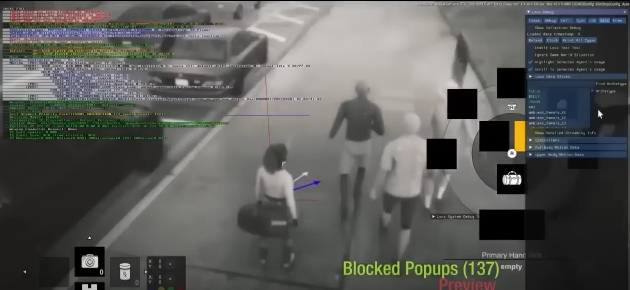
\includegraphics[height=0.4\textwidth]{rage_vector_math}
    \caption{Vectorial Math in RAGE Engine}
\end{figure}

\subsubsection*{Hybrid Models}

Unity represents a hybrid model, offering a free version with basic features and an open API, while advanced features require paid licenses. This approach balances accessibility with commercial viability, supporting widespread use and continuous innovation.

\subsection*{Open Software in this Project}

This project embraces open-source principles, making the game engine's source code publicly available to foster innovation and customization. This openness enhances the engine's versatility and encourages a community of contributors to drive its evolution.

